\vspace{12pt}
\section{Pulsed Laser Deposition of Thin Films} \label{section:PLD}
The technique of pulsed laser deposition (PLD) was used in this research to create thin films of barium zirconate based materials. PLD has been recognized over the past decade as a promising approach for producing thin films of ionic conductors. It produces consistent transfer of complex target stoichiometry to the thin films, and has delivered pinhole-free films of sub-micron thickness, which is essential in fuel-cell and electrolyzer applications that require leak-tight configurations regarding the gas feedstocks. Figure \ref{fig:PLD_Setup} provides a schematic of the PLD apparatus used to deposit our films. In PLD, a laser is shot at a rotating target inside a vacuum chamber, creating a highly ionized gaseous plume of target material which is directed onto a substrate.  Exposure of the substrate to the plume results in the growth of a thin film on the substrate surface. Rotation of the substrate allows for even distribution of deposited material. Heating the substrate provides energy for surface diffusion of the deposited material, which is vital to film crystallization. The pressure in the vacuum chamber and the atmosphere can be manipulated to affect the kinetic energy and the gas phase chemistry of the particles that eventually collide with the substrate. The laser energy density and pulse repetition rate can be adjusted to modify the number density, kinetic energy, and ionization of the particles in the plume. The large number of deposition parameters and their broad dynamic range allow exploration of different regimes of crystal growth with high potential for generating new thin film growth. 

\begin{figure}
    \centering
    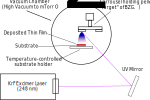
\includegraphics{Figures/PLD_2.pdf}
    \caption{Schematic of the apparatus used for pulsed laser deposition. A high-power pulsed laser is used for ablating a solid target, creating a plume of ejected species which subsequently deposits onto a perpendicularly placed substrate where thin film crystal growth takes place.}
    \label{fig:PLD_Setup}
\end{figure}
